\documentclass[
  11pt,
  letterpaper,
   addpoints,
   answers
  ]{exam}

\usepackage{../exercise-preamble}

\begin{document}

\noindent
\begin{minipage}{0.47\textwidth}

\includegraphics[width=\textwidth]{../fcfm_die}
\end{minipage}
\begin{minipage}{0.53\textwidth}
\begin{center} 
\large\textbf{Análisis de Sistemas Dinámicos y Estimación} (EL3204-2) \\
\large\textbf{Tarea 1} \\
\normalsize Prof.~Heraldo Rozas.\\
\normalsize Prof.~Aux.~Erik Saez - Maximiliano Morales
\end{center}
\end{minipage}

\vspace{0.5cm}
\noindent
\vspace{.85cm}

\begin{questions}
    %%%%%%%%%%%%%%%%%%%%%%%%%%%
    \question Considere el sistema de la siguiente figura, donde se tiene un carro atado a un resorte con un sensor de distancia, capaz de medir la distancia del carro a la pared. Suponga que existe una fuerza de fricción viscosa con la superficie $F_f$ de la forma $F_f = b_1 \dot{z} + b_2 (\dot{z}^2)$.
    \begin{figure}[h!]
        \centering
        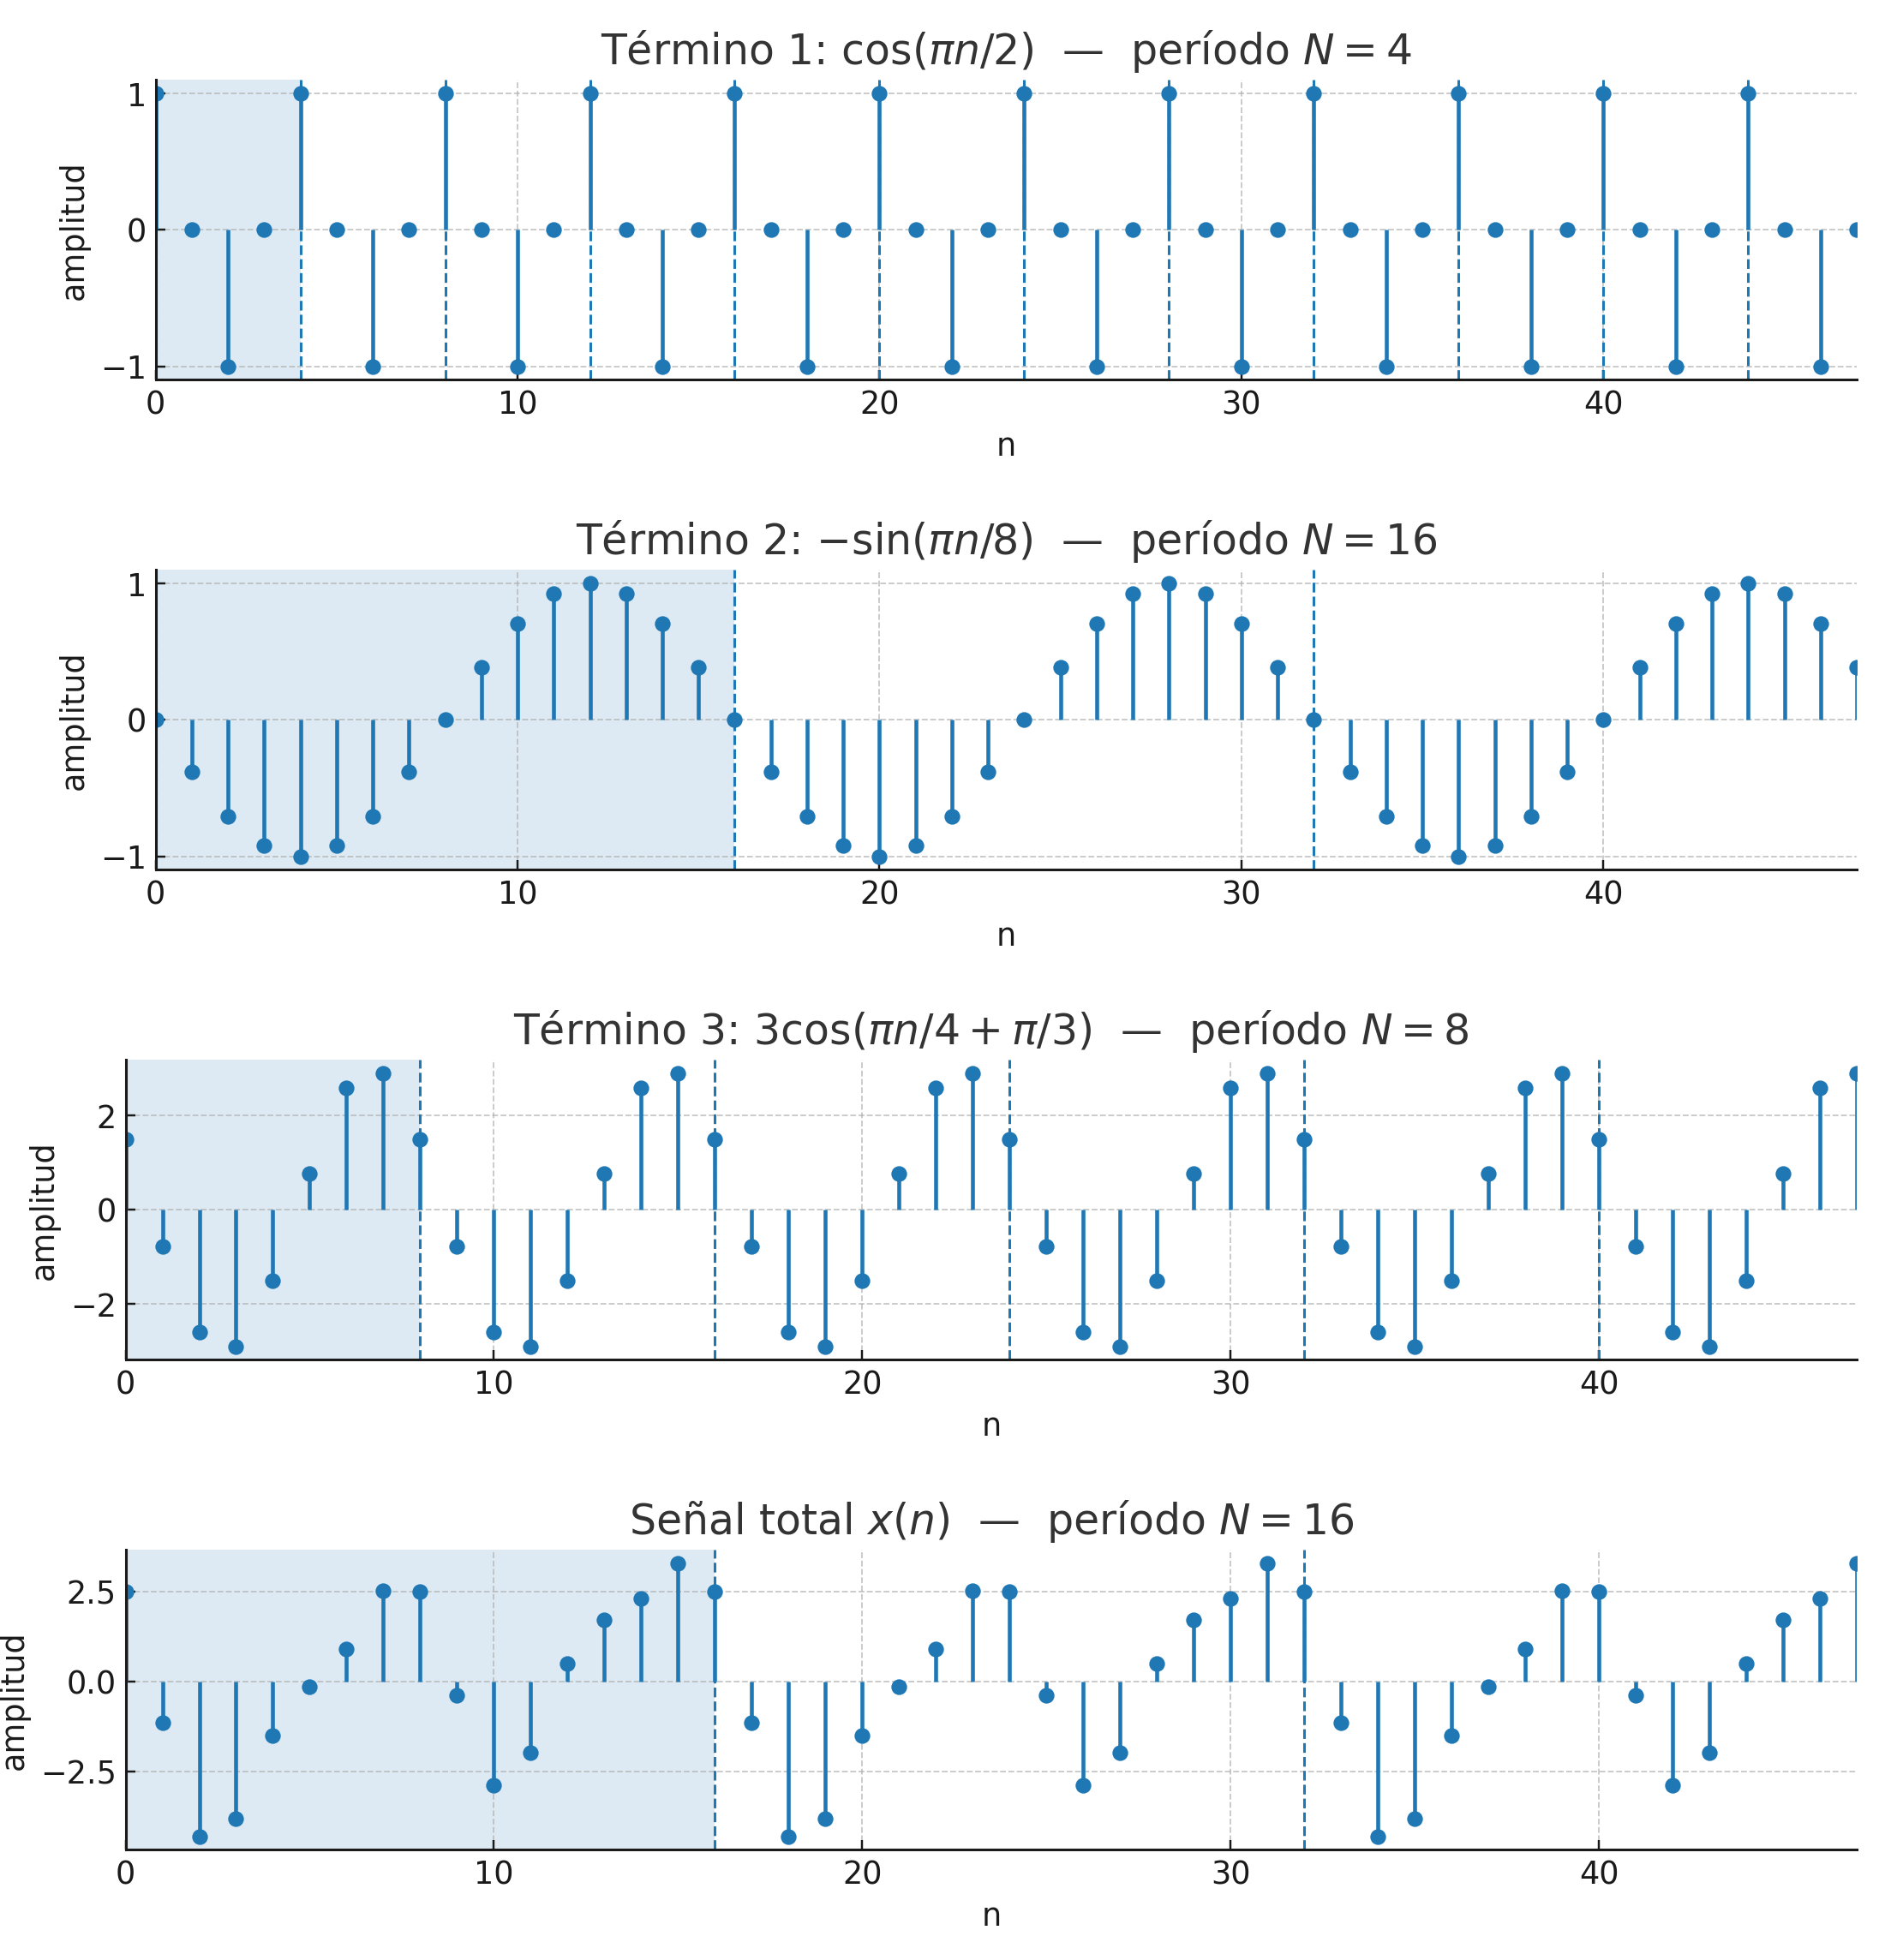
\includegraphics[width=0.45\textwidth]{Auxiliar_1_1}
    \end{figure}
    \begin{enumerate}
        \item Establezca hipótesis simplificatorias para el problema.
        \item Formule un modelo matemático del sistema que sea consistente con sus hipótesis.
        \item Encuentre el punto de operación que asegure $z = 1$ m.
    \end{enumerate}
    %%%%%%%%%%%%%%%%%%%%%%%%%%%
    \begin{solution}
    \subsection*{Resolucion 1.1}
        Para poder plantear un buen modelo, es necesario establecer hipótesis que simplifiquen el problema y lo hagan abordable. Estas hipótesis son muy importantes, ya que pueden complejizar o simplificar el problema cuanto sea necesario. Para este caso particular, algunas hipótesis que se pueden plantear para simplificar el problema son:
\begin{enumerate}
    \item El carro solamente se mueve \textbf{horizontalmente.}
    \item El resorte actúa en el \textbf{régimen lineal}, de acuerdo a la ley de Hooke.
    \item La constante elástica $k$ del resorte no varía, y su largo natural $l_0$ es 0.
    \item El roce es de la forma 
    \begin{equation}
        F_f = b_1 \dot{z} + b_2 \dot{z}^2.
    \end{equation}
    \item La fuerza $F(t)$ es conocida y varía en el tiempo.
\end{enumerate}
\subsection*{Resolucion 1.2}
Plantear un modelo matemático para un sistema físico se reduce, generalmente, a encontrar una ecuación diferencial que modele la dinámica del sistema. Para este caso particular, podemos utilizar segunda ley de Newton para obtener dicha ecuación diferencial.
\begin{equation}
    m\ddot{z} = F(t) - F_e - F_f, \tag{2}
\end{equation}
Donde $F_e$ corresponde a la fuerza elástica del resorte, y $F_f$ es la fuerza de roce. La fuerza elástica, por la segunda hipótesis, está dada por
\begin{equation}
    F_e = kz, \tag{3}
\end{equation}
por lo que la ecuación 2 es
\begin{equation}
    m\ddot{z} = F(t) - kz - b_1\dot{z} - b_2\dot{z}^2. \tag{4}
\end{equation}
Despejando $\ddot{z}$, tenemos que el modelo matemático es
\begin{equation}
    \ddot{z} = \frac{1}{m}F(t) - \frac{k}{m}z - \frac{b_1}{m}\dot{z} - \frac{b_2}{m}\dot{z}^2. \tag{5}
\end{equation}
\subsection*{Resolucion 1.3}
Para encontrar el punto de operación, el objetivo es determinar el valor de la entrada $F(t)$ de modo tal que se tenga $z = 1 \, \text{m}$. Implícitamente, al hablar de punto de operación se requiere estaticidad (a menos que se indique lo contrario), por lo que podemos asumir que $z$ no varía, indicando que $\dot{z} = \ddot{z} = 0$.

Podemos utilizar lo anteriormente mencionado sobre el modelo, imponiendo las condiciones indicadas y encontrando el valor de $F(t)$ que las satisfaga. Imponiendo $z = 1$, $\dot{z} = \ddot{z} = 0$ sobre la ecuación 5 tenemos
\begin{equation}
    0 = \frac{1}{m}F(t) - \frac{k}{m} \quad \Rightarrow \quad F(t) = k,
\end{equation}
por lo que el punto de operación es $F(t) = k$. Un aspecto importante a notar es que, para encontrar este punto de operación, asumimos que la fuerza $F(t)$ es constante en el tiempo. Más adelante dentro del ramo (y en otros ramos de la carrera) veremos que considerar una fuerza constante no siempre es lo ideal, sino que es posible diseñar una entrada particular para llegar a la condición de estaticidad más rápidamente.
    \end{solution}
    %%%%%%%%%%%%%%%%%%%%%%%%%%%
    \question Considere el siguiente péndulo apoyado en un carro móvil, el cual se desliza por una barra.
    \begin{enumerate}
        \item Establezca hipótesis simplificatorias.
        \item Formule un modelo matemático, que capture la dinámica del sistema.
        \item Identifique entradas, salidas y estados en su modelo.
        \item Linealice en torno a $\theta = \pi$.
    \end{enumerate}
    \begin{figure}[h]
        \centering
        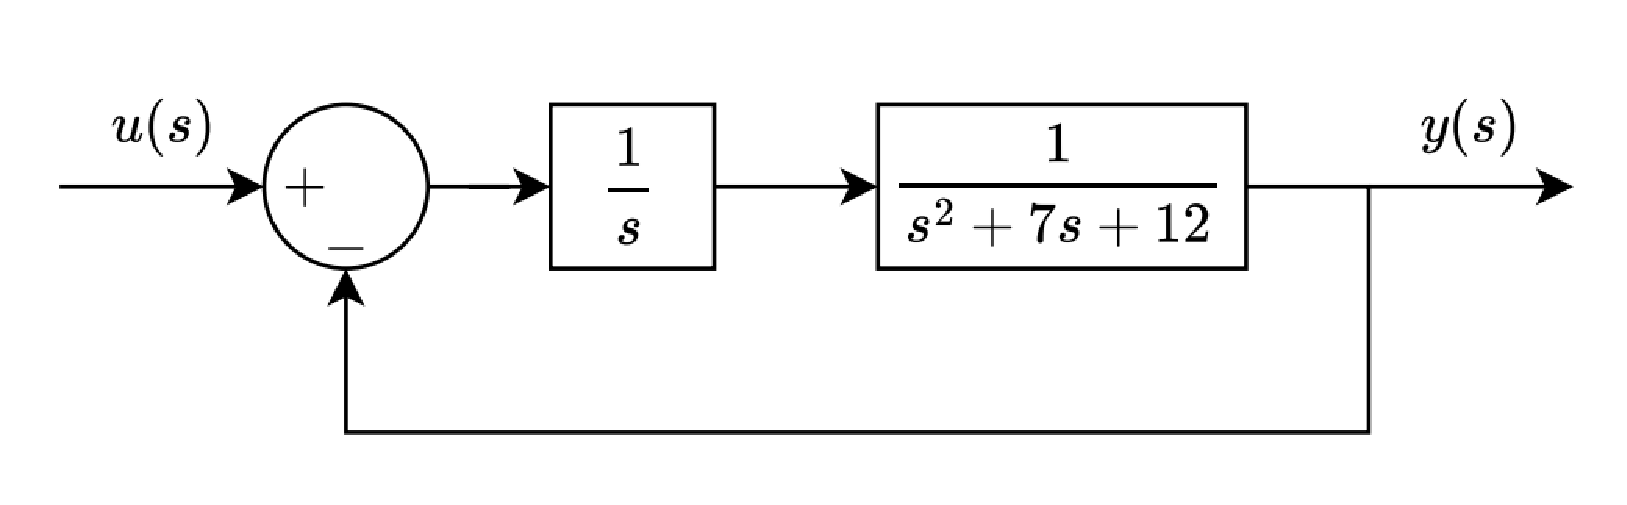
\includegraphics[width=0.5\textwidth]{Auxiliar_1_2}
    \end{figure}
%%%%%%%%%%%%%%%%%%%%%%%%%%%
\begin{solution}
\subsection*{Resolucion 2.1}
    Similar al ejercicio anterior, es necesario establecer buenas hipótesis simplificatorias para que el problema sea abordable. Algunas de estas hipótesis que podemos plantear son las siguientes:
\begin{enumerate}
    \item El carro tiene masa despreciable.
    \item La vara del péndulo no tiene masa.
    \item La vara del péndulo es rígida.
    \item La bola del péndulo es una masa puntual.
    \item No hay roce con el aire.
    \item Solamente existe movimiento en los dos ejes ilustrados.
\end{enumerate}
\subsection*{Resolucion 2.2}
Utilizando las hipótesis planteadas, podemos encontrar un modelo matemático. Para esto, si bien se podría utilizar la segunda ley de Newton para plantear una ecuación diferencial, al ser un péndulo este es un proceso engorroso: en cambio, utilizaremos mecánica Lagrangiana para plantear la ecuación diferencial.El Lagrangiano corresponde a $L = T - V$, con $T$ la energía cinética y $V$ la energía potencial, junto a la ecuación de Euler-Lagrange
\begin{equation}
    \frac{\partial L}{\partial q} - \frac{d}{dt} \left( \frac{\partial L}{\partial \dot{q}} \right) = 0, \tag{7}
\end{equation}
Donde es importante destacar que \textbf{q} representa la coordenada que estemos utilizando y por tanto segun el sistemas de coordenadas que se utilice se debera obtener su Lagrangiano asociado a cada componente.Es importante notar que la ecuación de Euler-Lagrange planteada de esa manera es válida si no existen pérdidas de energía en el sistema: si hubiesen fuerzas no conservativas, se deberían considerar dentro de la ecuación.Este supuesto es válido debido a la hipótesis de que no hay roce.Para calcular el Lagrangiano, debemos comenzar calculando la energía cinética.Dado que solamente la bola del péndulo tiene masa, este será el único componente con energía cinética.Si llamamos $x_p, y_p$ a la posición del péndulo, podemos notar que esta se puede escribir como
\begin{equation}
    x_p = x + l \sin \theta \quad y_p = -l \cos \theta,
\end{equation}
donde se asume que $y$ es positivo hacia arriba, que $y = 0$ corresponde a la ubicación de la barra, y que se tiene una distancia $x(t)$ desde el origen a la vertical del péndulo. Con estas posiciones, la energía cinética estará dada por
\begin{equation}
    T = \frac{1}{2} m \left( \dot{x}_p^2 + \dot{y}_p^2 \right). \tag{9}
\end{equation}
Calculando las derivadas, tenemos
\begin{equation}
    \dot{x}_p = \dot{x} + l \dot{\theta} \cos \theta \quad \dot{y}_p = l \dot{\theta} \sin \theta, \tag{10}
\end{equation}
donde los términos \(\dot{\theta}\) salen por la regla de la cadena (\textit{Es muy importante tener en consideración esto último, dado que \(\dot{\theta}\) también es una variable}). Utilizándolos para calcular la energía cinética, tenemos:
\begin{equation}
    T = \frac{1}{2} m \left( \dot{x}^2 + \dot{x} l \dot{\theta} \cos \theta + l^2 \dot{\theta}^2 \cos^2 \theta + l^2 \dot{\theta}^2 \sin^2 \theta \right). \tag{11}
\end{equation}
Podemos notar que:
\begin{equation}
    l^2 \dot{\theta}^2 \cos^2 \theta + l^2 \dot{\theta}^2 \sin^2 \theta = l^2 \dot{\theta}^2 (\cos^2 \theta + \sin^2 \theta) = l^2 \dot{\theta}^2, \tag{12}
\end{equation}
Luego:
\begin{equation}
    T = \frac{1}{2} m \left( \dot{x}^2 + 2 \dot{x} l \dot{\theta} \cos \theta + l^2 \dot{\theta}^2 \right) = \frac{1}{2} m \dot{x}^2 + m l \dot{x} \dot{\theta} \cos \theta + \frac{1}{2} m l^2 \dot{\theta}^2. \tag{13}
\end{equation}
Para la energía potencial, dado que el único componente que tiene masa es la bola del péndulo, solamente se tiene la contribución de su energía potencial gravitatoria. Además, dado que la vara es rígida, sabemos que no actúa como un resorte, y, por ende, no hay energía potencial elástica. Considerando todo esto, la energía potencial $V$ está dada por
\begin{equation}
    V = mg \cdot y_p = -mgl \cos \theta. \tag{14}
\end{equation}
Luego, el Lagrangiano es
\begin{equation}
    L = \frac{1}{2} m \left( \dot{x}^2 + 2 \dot{x} l \dot{\theta} \cos \theta + l^2 \dot{\theta}^2 \right) + mgl \cos \theta. \tag{15}
\end{equation}
Para poder considerar el Lagrangiano dentro de la ecuación de Euler-Lagrange, es necesario calcular las derivadas de cada término. Dado que estamos trabajando en coordenadas polares, sabemos que hay dos coordenadas, el radio \(r\) y el ángulo \(\theta\). Dado que \(r = l\) es constante, sabemos que no hay dinámica en la dirección radial, por lo que solamente nos interesa analizar la dinámica angular. Esto significa que debemos calcular las derivadas de \(L\) con respecto a \(\theta\) y \(\dot{\theta}\). Calculando las derivadas, tenemos
\begin{align}
    \frac{\partial L}{\partial \theta} &= -mgl \sin \theta - ml \dot{x} \sin \theta, \tag{20} \\
    \frac{\partial L}{\partial \dot{\theta}} &= ml^2 \dot{\theta} + ml \dot{x} \cos \theta. \tag{21}
\end{align}
Un punto importante notar a la hora de calcular las derivadas, es que, al derivar con respecto a \(\theta\), se debe tener en cuenta que \(\dot{\theta}\) no depende de \(\theta\), sino que solamente del tiempo. Lo mismo aplica a la hora de derivar con respecto a \(\dot{\theta}\), en donde \(\dot{\theta}\) actúa como una constante.
Luego, usando la ecuación 21 podemos tomar la derivada con respecto al tiempo, de lo que tenemos
\begin{align}
    \frac{d}{dt} \left( \frac{\partial L}{\partial \dot{\theta}} \right) 
    &= \frac{d}{dt} \left( ml^2 \dot{\theta} + ml \dot{x} \cos \theta \right) \tag{22}\\
    &= ml^2 \ddot{\theta} + ml \left( \dot{x} \cos \theta - \dot{x} \dot{\theta} \sin \theta \right)\\
    &= ml^2 \ddot{\theta} + ml \dot{x} \cos \theta - ml \dot{x} \dot{\theta} \sin \theta. \tag{23}
\end{align}
Insertando estos términos dentro de la ecuación de Euler-Lagrange, tenemos
\begin{align}
    \frac{\partial L}{\partial \theta} - \frac{d}{dt} \left( \frac{\partial L}{\partial \dot{\theta}} \right) &= 0 \tag{26}\\
    = -mgl \sin \theta - ml \dot{x} \sin \theta - ml^2 \ddot{\theta} - ml \ddot{x} \cos \theta + ml \dot{x} \dot{\theta} \sin \theta &= 0 \tag{27}\\
    = -mgl \sin \theta - ml^2 \ddot{\theta} - ml \ddot{x} \cos \theta &= 0. \tag{28}
\end{align}
Reordenando términos para despejar \(\ddot{\theta}\) en función del resto de variables, obtenemos
\begin{equation}
    \ddot{\theta} = -\frac{g}{l} \sin \theta - \frac{\cos \theta}{l} \ddot{x}, \tag{29}
\end{equation}
la cual corresponde a la ecuación diferencial que modela la dinámica del problema.
\subsection*{Resolucion 2.3}
Para identificar las entradas, debemos identificar aquellas variables que podemos manipular y que no dependen de la dinámica del problema. En este caso, podemos ver que \(\ddot{x}\), correspondiente a la aceleración del carro, es una variable libre del problema la cual no depende del resto de variables, por lo que podemos considerarla como la entrada al sistema.\\\\
Con respecto a la salida, esta es la variable que más libertad entrega a quien modela, dado que depende del fenómeno de interés. En general, se puede considerar una variable de salida cualquiera de los sensores que se están utilizando para medir las variables, por lo que estos valores medidos por los sensores podrían considerarse las salidas. Sin embargo, en este problema no se indican los sensores presentes, por lo que asumiremos que cualquier variable es salida, por lo que, arbitrariamente, se escoge que \(\theta\) es la salida.\\\\
Para reforzar el punto de la salida, podemos imaginarnos distintos casos hipotéticos sobre el sistema planteado en esta pregunta. Por ejemplo, podríamos instalar un motor en el carro al cual se encuentre conectada la vara del péndulo, y podríamos instalar un sensor que mida el voltaje que sale del motor. Al hacer esto, dado que el voltaje del motor será proporcional a la salida, en esencia tendríamos que la salida es \(\theta\). Otra posibilidad es que, en vez de los sensores planteados, podríamos instalar una IMU (Inertial Measurement Unit) en la bola del péndulo, el cual mide la aceleración de la bola en coordenadas cartesianas, por lo que tendríamos dos salidas \(\dot{x}_p\) y \(\dot{y}_p\).\\\\
Finalmente, las últimas variables a indicar son los estados. Los estados corresponden a aquellas variables que tienen incidencia directa sobre la dinámica del sistema planteado. Una forma práctica de verlo es que cualquier diferencial que modele al sistema: si el sistema está modelado por una edo de orden n, entonces todas las derivadas de menor orden (incluyendo el orden 0, que corresponde a la variable sin derivar) van a corresponder a los estados del sistema\footnote{Otra forma útil de verlo es que los estados van a corresponder a todas aquellas variables para las cuales se debe indicar una condición inicial.}. En el problema planteado, dado que el modelo es una edo de orden 2, sabemos que las derivadas de orden 1 (\(\dot{\theta}\)) y orden 0 (\(\theta\)) serían los estados del sistema.
\subsection*{Resolucion 2.4}
La linealización es un proceso en el cual generamos una aproximación lineal de la edo que modela al sistema, utilizando los primeros términos de la serie de Taylor.
Para esto, notemos que podemos escribir la ecuación 29 como
\begin{equation}
    \ddot{\theta} = f(\theta, u), \tag{30}
\end{equation}
tal que
\begin{equation}
    f(\theta, u) = -\frac{g}{l} \sin \theta - \frac{\cos \theta}{l} u, \tag{31}
\end{equation}
Es importante notar que denotamos \(u = \ddot{x}\) para abreviar. Luego, la idea de linealizar es calcular la serie de Taylor de la función \(f(\theta, u)\) en torno a un cierto punto \((\bar{\theta}, \bar{u})\), de modo que el sistema linealizado sería una \textbf{buena aproximación del sistema original en torno al punto \((\bar{\theta}, \bar{u})\)}.

Calculando la serie de Taylor de la función \(f(\theta, u)\) en torno a \((\bar{\theta}, \bar{u})\) tenemos
\begin{equation}
    f(\theta, u) = f(\bar{\theta}, \bar{u}) + (\theta - \bar{\theta}) \frac{\partial f(\bar{\theta}, \bar{u})}{\partial \theta} + (u - \bar{u}) \frac{\partial f(\bar{\theta}, \bar{u})}{\partial u} + O((\theta - \bar{\theta})^2) + O((u - \bar{u})^2), \tag{32}
\end{equation}
donde \(O((\theta - \bar{\theta})^2) y O((u - \bar{u})^2)\) contienen los términos de mayor orden.Dado que buscamos una aproximación lineal, podemos omitir estos términos de mayor orden, de modo que tenemos
\begin{equation}
    f(\theta, u) \approx f(\bar{\theta}, \bar{u}) + (\theta - \bar{\theta}) \frac{\partial f(\bar{\theta}, \bar{u})}{\partial \theta} + (u - \bar{u}) \frac{\partial f(\bar{\theta}, \bar{u})}{\partial u}, \tag{33}
\end{equation}
donde, para abreviar, denotamos
\begin{equation}
  \quad f_{\theta} = \frac{\partial f(\bar{\theta}, \bar{u})}{\partial \theta}, \quad f_{u} = \frac{\partial f(\bar{\theta}, \bar{u})}{\partial u}. \tag{34}
\end{equation}

Luego, podemos reordenar los términos como
\begin{equation}
    f(\theta, u) - f(\bar{\theta}, \bar{u}) = (\theta - \bar{\theta}) f_{\theta} (\bar{\theta}, \bar{u}) + (u - \bar{u}) f_{u} (\bar{\theta}, \bar{u}), \tag{35}
\end{equation}
por lo que, si definimos \(\tilde{\theta} := \theta - \bar{\theta}, \tilde{u} := u - \bar{u}\), considerando que \(\ddot{\theta} = f(\theta, u)\) y definiéndose \(\tilde{\ddot{\theta}} := \ddot{\theta} - f (\bar{\theta}, \bar{u})\) tenemos
\begin{equation}
    \tilde{\ddot{\theta}} = f_{\theta} (\bar{\theta}, \bar{u}) \tilde{\theta} + f_{u} (\bar{\theta}, \bar{u}) \tilde{u}, \tag{36}
\end{equation}
donde podemos ver que los términos \(f_{\theta} (\bar{\theta}, \bar{u})\) y \(f_{u} (\bar{\theta}, \bar{u})\) solamente dependen del punto de linealización, por lo que son constantes. Así, el nuevo modelo corresponde a una EDO lineal.

Finalmente, utilicemos esto para obtener la linealización del sistema. En este caso, se nos indica que queremos linealizar en torno a \(\theta = \pi\), por lo que tenemos \(\bar{\theta} = \pi\). Dado que no se nos indica el valor de entrada en torno a la cual queremos linealizar, podemos asumir \(\bar{u} = 0\). Luego, calculemos todas las derivadas necesarias para obtener la linealización. Haciéndolo, tenemos
\begin{equation}
    f_{\theta} (\theta, u) = \frac{\partial}{\partial \theta} \left( -\frac{g}{l} \sin \theta - \frac{\cos \theta}{l} u \right) = -\frac{g}{l} \cos \theta + \frac{\sin \theta}{l} u \Rightarrow f_{\theta} (\bar{\theta}, \bar{u}) = -\frac{g}{l}, \tag{37}
\end{equation}
\begin{equation}
    f_{u} (\theta, u) = \frac{\partial}{\partial u} \left( -\frac{g}{l} \sin \theta - \frac{\cos \theta}{l} u \right) = -\frac{\cos \theta}{l} \Rightarrow f_{u} (\bar{\theta}, \bar{u}) = -\frac{1}{l}, \tag{38}
\end{equation}
por lo que el modelo linealizado en torno a \(\theta = \pi\) es de la forma
\begin{equation}
    \tilde{\ddot{\theta}} = -\frac{g}{l} \tilde{\theta} - \frac{1}{l} \tilde{u}. \tag{39}
\end{equation}
\end{solution}
%%%%%%%%%%%%%%%%%%%%%%%%%%%
\question \textbf{(Propuesto)}Considere el proceso de elaboración del típico alimento chileno conocido como ``manjar'', de sabor similar (pero no idéntico) al ``dulce de leche'' argentino (ver figura 2). En dicho proceso se sumerge un recipiente metálico (sellado) que contiene leche condensada en una olla con agua. Posteriormente, se procede a calentar el agua, lo que conlleva un suave proceso de cocción de la leche condensada. Sea $Q(t)$ una medida de calor aplicado para calentar el agua de la olla.
\begin{figure}[h!]
    \centering
    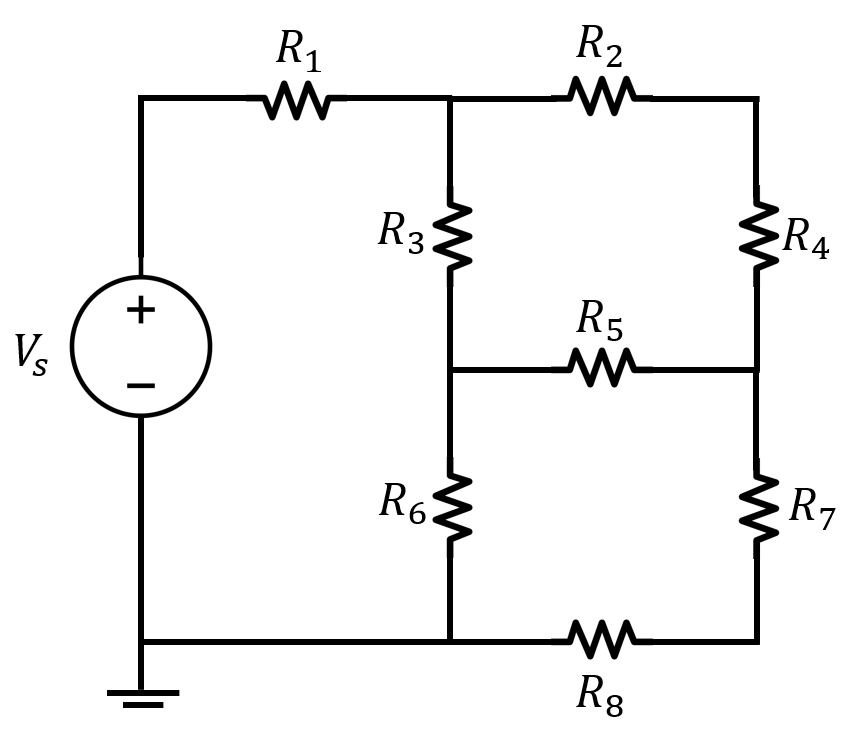
\includegraphics[width=0.3\linewidth]{Auxiliar_1_3}
    \caption{Proceso elaboración manjar}
\end{figure}
\begin{enumerate}
    \item Obtenga un modelo matemático que caracterice la evolución de las temperaturas en el tiempo. Enumere y describa todas las hipótesis simplificatorias utilizadas para obtener dicho modelo.
    \item Indique al menos 8 características principales que tendrá su modelo resultante y realice una clasificación de todas las variables del sistema indicando sus unidades en el sistema MKS. En particular refiérase a las variables de estado y a los estados cero, de referencia y equilibrio.
    \item Suponiendo que las entradas al sistema es (son) constante(s), obtenga un modelo linealizado en torno a un punto de operación arbitrario.
\end{enumerate}
%%%%%%%%%%%%%%%%%%%%%%%%%%%
\begin{solution}
    Para modelar este sistema, utilizaremos las siguientes hipótesis simplificatorias:

\begin{enumerate}
    \item La olla está llena de agua y está herméticamente cerrada.
    \item El agua tiene densidad $\rho$ y volumen $V$ constantes.
    \item Las masas $M$ y $m$, del manjar y del tarro, respectivamente, son constantes.
    \item La temperatura está uniformemente distribuida.
    \item Los calores específicos de cada medio son constantes.
    \item Las paredes permiten el intercambio de calor con el ambiente (no son adiabáticas).
\end{enumerate}

donde es importante notar que el modelo obtenido depende directamente de las hipótesis utilizadas, por lo que si se usan otras hipótesis el modelo puede cambiar. Con esto, los parámetros asociados a cada medio se pueden ver en la tabla
\begin{center}
    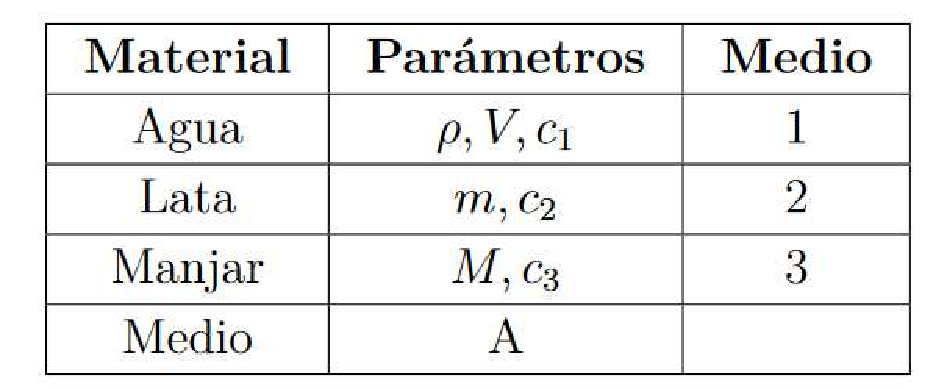
\includegraphics[width=0.4\textwidth]{Auxiliar_1_4}
    \captionof{figure}{Tabla de parámetros}
  \end{center}
Por ecuación de Newton, tenemos:
\begin{align}
    q_{ij} &= h_{ij}A_{ij} (T_i - T_j)
    \end{align}    
Donde $q_{ij}$ es el flujo de calor desde el medio $i$ hasta el medio $j$, $h_{ij}$ es el coeficiente de transferencia desde el medio $i$ hasta el medio $j$, $A_{ij}$ es el área de contacto entre el medio $i$ y el medio $j$, y $T_i$, $T_j$ son las temperaturas del medio $i$ y $j$, respectivamente.
Luego, por balance térmico tenemos:
\begin{align}
    \frac{dH_1}{dt} &= Q + q_{A1} + q_{21} \tag{13} \\
    \frac{dH_2}{dt} &= q_{12} + q_{32} \tag{14} \\
    \frac{dH_3}{dt} &= q_{23} \tag{15}
    \end{align}    
con $Q$ el calor emitido por la cocina, y $H_i$ la entalpía del medio $i$, dada por:
\begin{align}
    H_i &= m_i c_i T_i \tag{17}
    \end{align}
Considerando esto, podemos realizar el balance térmico en cada medio. En el agua se tiene $m_1 = \rho V$, por lo que, de acuerdo a la ecuación (13), tenemos:
\begin{align}
    \rho V c_1 \frac{dT_1}{dt} &= Q + h_{A1}A_{A1} (T_A - T_1) + h_{21}A_{21} (T_2 - T_1) \tag{18} \\
    \Rightarrow \frac{dT_1}{dt} &= \frac{Q + h_{A1}A_{A1} (T_A - T_1) + h_{21}A_{21} (T_2 - T_1)}{\rho V c_1} \tag{19}
    \end{align}
Para la lata, considerando que su masa es $m$, de acuerdo a su ecuación (14) tenemos:
\begin{align}
    mc_2 \frac{dT_2}{dt} &= h_{12}A_{12} (T_1 - T_2) + h_{32}A_{32} (T_3 - T_2) \tag{20} \\
    \Rightarrow \frac{dT_2}{dt} &= \frac{h_{12}A_{12} (T_1 - T_2) + h_{32}A_{32} (T_3 - T_2)}{mc_2} \tag{21}
\end{align}
Finalmente, para el manjar, considerando que su masa es $M$, por la ecuación (15) tenemos
\begin{align}
    MC_3 \frac{dT_3}{dt} &= h_{23}A_{23} (T_2 - T_3) \tag{22} \\
    \Rightarrow \frac{dT_3}{dt} &= \frac{h_{23}A_{23} (T_2 - T_3)}{MC_3} \tag{23}
\end{align}
Con las ecuaciones (19), (21) y (23) tenemos un modelo matemático para las variaciones de temperatura en cada medio.
\subsection*{Resolución 3.2}
A continuación entregaremos 8 características principales del modelo:
\begin{enumerate}
    \item Es un modelo basado en leyes de conservación de energía.
    \item Es de parámetros concentrados, dado que se realizó el supuesto de que la temperatura se distribuye uniformemente, por lo que no depende de la posición.
    \item Es dinámico, dado que la temperatura de cada medio varía en función del tiempo.
    \item Es artificial, dado que la situación es creada y manipulada por los humanos.
    \item Es determinístico, ya que no hay variables aleatorias en el modelo.
    \item Es monovariable, ya que hay una sola variable de entrada (el calor $Q$) y una sola variable de salida (en este caso, la temperatura del manjar $T_3$).
    \item Es de tiempo continuo, ya que presenta derivadas con respecto al tiempo.
    \item Es causal, dado que el estado actual solamente le importan los valores pasados, no los valores futuros.
\end{enumerate}

Las variables utilizadas dentro del modelo, además de sus unidades en el sistema MKS, son las siguientes:

\begin{itemize}
    \item $T_i$ [K]: Temperatura del medio $i$, correspondiente a las variables de estado del sistema. En general, se define un vector $\mathbf{T} = (T_1, T_2, T_3)$ el cual corresponderá a la única variable de estado.
    \item $Q(t)$ [J]: Calor de entrada entregado a la olla. Corresponde a la variable de entrada al sistema.
\end{itemize}

Obtengamos, además, los estados cero, de referencia y de equilibrio. Para obtener el estado cero $T_0$, comencemos notando que se espera tal que la salida es nula: dado que la salida corresponde a la temperatura $T_3$ del manjar, para que esta sea nula se debe cumplir que $T_3 = 0$, por lo que $T_0 = (T_1, T_2, 0)$, con $T_1, T_2$ temperaturas no necesariamente nulas.
Para el estado de equilibrio, debemos notar que este corresponde a un estado que, bajo entrada cero, se mantiene indefinidamente en el tiempo. Dado que se mantiene en el tiempo, esto significa que no cambia y, por lo tanto, su derivada temporal es nula. Considerando esto, para obtener el estado de equilibrio igualamos las derivadas en las ecuaciones (19), (21) y (23) a 0, utilizamos $Q = 0$ (ya que es a entrada cero) y obtenemos $T_1$, $T_2$ y $T_3$.
\begin{align}
    0 &= 0 + h_{A1}A_{A1} (T_A - T_1) + h_{21}A_{21} (T_2 - T_1) \Rightarrow T_1 = T_2 = T_A \tag{24} \\
    0 &= h_{12}A_{12} (T_1 - T_2) + h_{32}A_{32} (T_3 - T_2) \Rightarrow T_1 = T_2 = T_3 \tag{25} \\
    0 &= \frac{h_{23}A_{23} (T_2 - T_3)}{MC_3} \Rightarrow T_2 = T_3 \tag{26}
\end{align}
Esto permite ver que el estado de equilibrio $T_e$ es aquel donde todas las temperaturas son la temperatura ambiente: es decir, $T_e = (T_A, T_A, T_A)$.

En efecto, de la ecuación (23) podemos deducir que $T_3 \rightarrow T_2$. Considerando esto, en la ecuación (21), dado que $T_3$ converge a $T_2$ su resta tenderá a 0, lo que implicaría $T_2 \rightarrow T_1$. A su vez, esto llevaría a que, en la ecuación (19), y considerando que $Q = 0$ dado que se analiza el caso de entrada cero, $T_1$ converja a $T_A$, indicando que todas las temperaturas convergen a la temperatura ambiente y, por lo tanto, $T_l = (T_A, T_A, T_A)$ es el estado de referencia.

Cuando se analizan los distintos estados de un sistema, resulta útil verificar que estos tienen sentido con la teoría física detrás del problema. En este caso, el hecho de que el estado cero corresponda a $(T_1, T_2, 0)$ es consistente con el hecho de que la salida es la tercera temperatura, por lo que basta que esta sea nula para que la salida también lo sea. Por otra parte, el hecho de que el estado de equilibrio y estado de referencia correspondan a aquel donde todas las temperaturas son la temperatura ambiente también es consistente con nuestra intuición detrás del problema: si dejamos un sistema a alta temperatura expuesto al medio, esperamos que eventualmente este le entregue todo su calor, equilibrando las temperaturas. Además, habiendo llegado a este estado no esperamos que, espontáneamente, las temperaturas varíen.
\subsection*{Resolución 3.3}
Para linearizar, consideremos un punto de operación arbitrario $T^* = (T_1^*, T_2^*, T_3^*)$ sobre el cual queremos linearizar el sistema. Si consideramos las funciones
\begin{align}
    \frac{dT_1}{dt} &= f_1(T) \tag{27} \\
    \frac{dT_2}{dt} &= f_2(T) \tag{28} \\
    \frac{dT_3}{dt} &= f_3(T) \tag{29}
\end{align}
podemos linearizarlas considerando:
\begin{align}
    f_i(T) &\approx f_i(T^*) + \frac{\partial f_i}{\partial T_1}\Big|_{T^*} (T_1 - T_1^*) + \frac{\partial f_i}{\partial T_2}\Big|_{T^*} (T_2 - T_2^*) + \frac{\partial f_i}{\partial T_3}\Big|_{T^*} (T_3 - T_3^*) \tag{30}
\end{align}
Al calcular cada uno de estos términos, tenemos
\begin{align}
    f_1(T) &\approx Q + h_{A1}A_{A1} (T_A - T_1^*) + h_{21}A_{21} (T_2^* - T_1^*) \nonumber \\
    &\quad - \frac{h_{A1}A_{A1} + h_{21}A_{21}}{\rho V c_1} (T_1 - T_1^*) + \frac{h_{21}A_{21}}{\rho V c_1} (T_2 - T_2^*) \tag{31} \\
    f_2(T) &\approx \frac{h_{12}A_{12} (T_1^* - T_2^*) + h_{32}A_{32} (T_3^* - T_2^*)}{mc_2} \nonumber \\
    &\quad + \frac{h_{12}A_{12}}{mc_2} (T_1 - T_1^*) - \frac{h_{12}A_{12} + h_{32}A_{32}}{mc_2} (T_2 - T_2^*) \nonumber \\
    &\quad + \frac{h_{32}A_{32}}{mc_2} (T_3 - T_3^*) \tag{32} \\
    f_3(T) &\approx \frac{h_{23}A_{23} (T_2^* - T_3^*)}{MC_3} + \frac{h_{23}A_{23}}{MC_3} (T_2 - T_2^*) - \frac{h_{23}A_{23}}{MC_3} (T_3 - T_3^*) \tag{33}
    \end{align}    
Reordenando términos, es posible ver que tanto $f_1(T)$, $f_2(T)$ y $f_3(T)$ llegan a sus expresiones originales: es decir, el sistema linearizado es idéntico al original. Esto ocurre debido a que, originalmente, las ecuaciones del sistema ya eran lineales, por lo que linearizar no tiene ningún efecto sobre estas.    

    
\end{solution}
\end{questions}
\newpage
%%%%%%%%%%%%%%%%%%%%%%%%%%%
\section{Resumen}
\begin{itemize}
    \item \textbf{Ecuación de Euler Lagrange}
    \[
    \frac{\partial L}{\partial q} - \frac{d}{dt} \frac{\partial L}{\partial \dot{q}} = 0 \tag{1}
    \]
    donde $L = T - V$, con $T$ energía cinética y $V$ energía potencial.
    \item \textbf{Estado cero} Un estado cero $x_0 \in \Sigma$ de un sistema es tal que la salida $y(t)$ cumple que
    \[
    y(t) = \mathcal{A}(x_0, 0) = 0 \tag{2}
    \]
    En términos sencillos: es una condición inicial tal que, para entrada cero, la salida es cero (dado que la salida depende del planteamiento del problema, el estado cero también lo hará).

    \item \textbf{Estado tierra} Un estado tierra $x_t \in \Sigma$ de un sistema es tal que
    \[
    \forall x_0 \in \Sigma, \lim_{t \to \infty} \mathcal{B}(x_0, 0) = x_t \tag{3}
    \]
    Es decir, el estado tierra es tal que, \textbf{PARA TODA CONDICIÓN INICIAL} y con entrada cero, el sistema converge al estado tierra.

    \item \textbf{Estado equilibrio} Un estado equilibrio $x_e \in \Sigma$ es tal que
    \[
    x_e = \mathcal{B}(x_e, 0) \tag{4}
    \]
    Esto significa que, bajo entrada cero, si el sistema está en estado equilibrio entonces se quedará por siempre en este.

    \item \textbf{Clasificación de sistemas} Algunas perspectivas desde las que podemos clasificar un sistema se pueden ver en la siguiente tabla:
\end{itemize}

\begin{table}[h!]
\centering
\begin{tabular}{|l|l|}
\hline
\textbf{Punto de vista} & \textbf{Clasificación} \\ \hline
Origen & Natural, Artificial \\ \hline
Naturaleza & Determinísticos, Aleatorios \\ \hline
Número de variables & Monovariables, Multivariables \\ \hline
Continuidad de variables & Discreto, Continuo \\ \hline
Comportamiento espacial & Variables concentradas, Variables Distribuidas \\ \hline
Comportamiento temporal & Variable, Invariable \\ \hline
Linealidad de variables & Lineal, No lineal \\ \hline
Realizabilidad & Causales, Anticipativos \\ \hline
\end{tabular}
\end{table}

\begin{itemize}
    \item \textbf{Linealización} Dado un sistema caracterizado por
    \[
    \dot{x} = f(x, u) \tag{5}
    \]
    si linealizamos en torno a un punto $\bar{x}, \bar{u}$ entonces
    \[
    \dot{\tilde{x}} = \frac{\partial f}{\partial x}\Big|_{\bar{x}, \bar{u}} \tilde{x} + \frac{\partial f}{\partial u}\Big|_{\bar{x}, \bar{u}} \tilde{u} \tag{6}
    \]
    con $\tilde{x} := x - \bar{x}$ y $\tilde{u} := u - \bar{u}$.
\end{itemize}
\end{document}